\epigraph{``I almost wish I hadn't gone down that rabbit-hole, and yet it's rather curious, you know, this sort of life!''}{\textit{Lewis Carroll\\ Alice's Adventures in Wonderland}}

\noindent \textbf{1 - Tale of the White Rabbit \cite{tale}}

\noindent ---~ \textbf{Fox:} ``What are you working on?''

\noindent ---~ \textbf{Rabbit:} ``My thesis.''

\noindent ---~ \textbf{Fox:} ``Hmmm. What's it about?''

\noindent ---~ \textbf{Rabbit:} ``Oh, I'm writing about how rabbits eat foxes''

\noindent ---~ \textbf{Fox:} ``That's ridiculous! Any fool knows that rabbits don't eat foxes''

\noindent ---~ \textbf{Rabbit:} ``Sure they do, and I can prove it. Come with me.''

They both disappear into the rabbit's burrow. After a few minutes, the rabbit returns, alone, to his typewriter and resumes typing.

\textbf{Scene inside the rabbit's burrow:} In one corner, there is a pile of fox bones. On the other side of the room, a huge lion is belching and picking his teeth. It doesn't matter what you choose for a thesis subject. It doesn't matter what you use for data. What does matter is who you have for a thesis advisor.

Following the tale of the white rabbit, I was advised by Ashutosh Saxena and He was flanked by Silvio Savarese. I am grateful to both of them for their scientific contribution, as well as allowing me to pursue my own ideas and patiently supporting me during the process. I am also thankful to my thesis committee members Emin G\"{u}n Sirer and David Mimno for their useful comments and suggestions. 

\noindent \textbf{2 - Down the Rabbit Hole @ Cornell}
First of all, I am grateful to Cornell Robot Learning Lab for creating a productive and fun environment both in Cornell and Stanford. I would like to thank my all officemates Ian Lenz, Ashesh Jain, Dipendra Misra and Jae Sung for all the discussions and fun we had, Hema Koppula for all the guidance and help, and Ian Lenz and Chenxia Wu for their support and friendship.

I am thankful to everyone who made me feel like at home in New York State. Especially, members of red tigers trivia team Ken Yancey, Breana Branham and Sean Rice, my juggling and magic partner Tayyar Rezayev, the Cornell Tech crew Stephanie Hyland, Neel Madhukar, Faisal Alquaddoomi and Natalie Davidson, and last but not least Turks of Cornell: Sinem Unal, Sevi Baltaoglu and Melik Turker.

\begin{wrapfigure}{r}{0.25\textwidth}
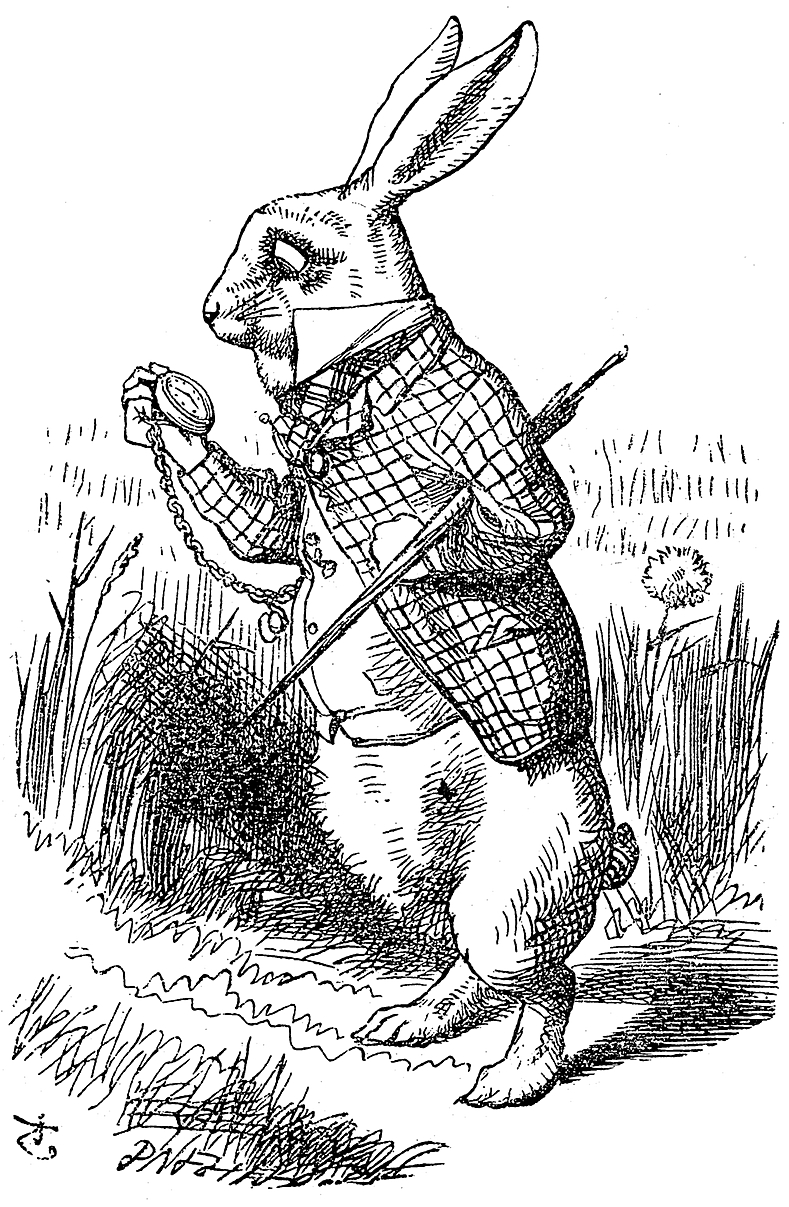
\includegraphics[width=0.24\textwidth]{alice.png}
\caption{The White Rabbit \cite{aiw}}
\end{wrapfigure}

\noindent \textbf{3 - A Mad Tea-Party @ Stanford}
I am grateful to Amir Zamir for countless impromptu discussions about life and science, and his guidance and help, Hyun Oh Song for his help in formalizing my ideas and Iro Armeni for her patience and understanding during our collaboration. I also had a chance to mentor two amazing undergrads during my PhD Hope Casey Allen and Jay Hack. I learned a lot from our discussions and hope to same for them. I am also grateful to all members of CVGL for their friendship, Alex Alahi, Amir Abbas, Yu Xiang, Chris Choy, Kevin and Kuang. I am also grateful to Hakan Inan for all the discussions we had about math. 

I am also thankful to everyone who converted this crazy tea-party of silicon valley into a joyful experience. Ilbey, Saumitro, Jonathan Ho, Shane and Rebecca; thanks a lot for your friendship. Finally, I am also grateful to one of the most beautiful places in the world -Dolores Park-

\noindent \textbf{4 - Queen of Hearts $\varheart$}
% Zehra, Mom, Dad, Umut
\iffalse
\noindent ---~ \textbf{Lion:} ``Hello, Fox. Why are you looking so gloomy?''

\noindent ---~ \textbf{Fox:} ``It's been like this all week. First my cub got sick, then the car started making a funny noise, and last night I accidently put my watch through the washing machine and it quit working.''

\noindent ---~ \textbf{Lion:} ``Well, I can't do much about the child or the car, but I can fix your watch for you.''

\noindent ---~ \textbf{Fox:} ``That'll be the day. You with your big claws? You would have trouble picking up the watch, let alone fixing the insides. You'll just break it even worse than it already is. I'd better take it into town.''

\noindent ---~ \textbf{Lion:} ``Let me take it into my den for a couple minutes. You'll be suprized.''

So he disappears into his den with the watch. A few minutes later he returns: the watch is fixed.

\textbf{Scene inside the lion's den:} In one corner, next to the coffee machine, is a smug-looking lion lying on a couch cleaning his fur. In a second corner, there are seven industrious rabbits surrounded by tiny parts and precision tools.  It doesn't matter whether you can write working programs or prove theorems. It doesn't matter whether you can do a slick demo or generate pretty pictures. What really matters is whether your graduate students can.
\fi 
